% Created by tikzDevice version 0.12.6 on 2024-03-27 11:38:36
% !TEX encoding = UTF-8 Unicode
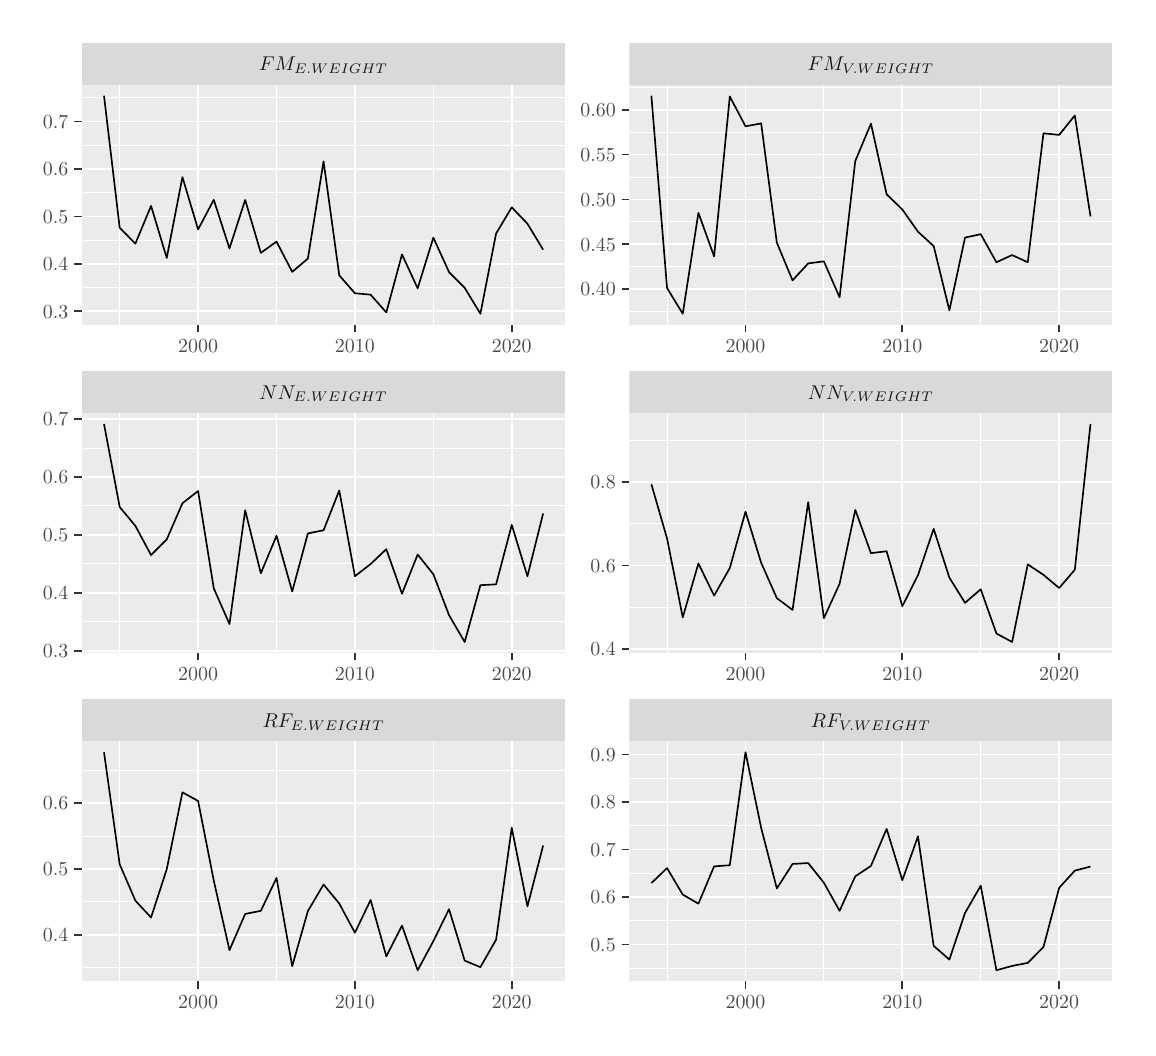
\begin{tikzpicture}[x=1pt,y=1pt]
\definecolor{fillColor}{RGB}{255,255,255}
\path[use as bounding box,fill=fillColor,fill opacity=0.00] (0,0) rectangle (397.48,361.35);
\begin{scope}
\path[clip] (  0.00,  0.00) rectangle (397.48,361.35);
\definecolor{drawColor}{RGB}{255,255,255}
\definecolor{fillColor}{RGB}{255,255,255}

\path[draw=drawColor,line width= 0.6pt,line join=round,line cap=round,fill=fillColor] (  0.00,  0.00) rectangle (397.48,361.35);
\end{scope}
\begin{scope}
\path[clip] ( 19.65,254.04) rectangle (194.19,340.69);
\definecolor{fillColor}{gray}{0.92}

\path[fill=fillColor] ( 19.65,254.04) rectangle (194.19,340.69);
\definecolor{drawColor}{RGB}{255,255,255}

\path[draw=drawColor,line width= 0.3pt,line join=round] ( 19.65,267.42) --
	(194.19,267.42);

\path[draw=drawColor,line width= 0.3pt,line join=round] ( 19.65,284.57) --
	(194.19,284.57);

\path[draw=drawColor,line width= 0.3pt,line join=round] ( 19.65,301.72) --
	(194.19,301.72);

\path[draw=drawColor,line width= 0.3pt,line join=round] ( 19.65,318.87) --
	(194.19,318.87);

\path[draw=drawColor,line width= 0.3pt,line join=round] ( 19.65,336.02) --
	(194.19,336.02);

\path[draw=drawColor,line width= 0.3pt,line join=round] ( 33.25,254.04) --
	( 33.25,340.69);

\path[draw=drawColor,line width= 0.3pt,line join=round] ( 89.92,254.04) --
	( 89.92,340.69);

\path[draw=drawColor,line width= 0.3pt,line join=round] (146.59,254.04) --
	(146.59,340.69);

\path[draw=drawColor,line width= 0.6pt,line join=round] ( 19.65,258.85) --
	(194.19,258.85);

\path[draw=drawColor,line width= 0.6pt,line join=round] ( 19.65,276.00) --
	(194.19,276.00);

\path[draw=drawColor,line width= 0.6pt,line join=round] ( 19.65,293.15) --
	(194.19,293.15);

\path[draw=drawColor,line width= 0.6pt,line join=round] ( 19.65,310.30) --
	(194.19,310.30);

\path[draw=drawColor,line width= 0.6pt,line join=round] ( 19.65,327.45) --
	(194.19,327.45);

\path[draw=drawColor,line width= 0.6pt,line join=round] ( 61.58,254.04) --
	( 61.58,340.69);

\path[draw=drawColor,line width= 0.6pt,line join=round] (118.25,254.04) --
	(118.25,340.69);

\path[draw=drawColor,line width= 0.6pt,line join=round] (174.92,254.04) --
	(174.92,340.69);
\definecolor{drawColor}{RGB}{0,0,0}

\path[draw=drawColor,line width= 0.6pt,line join=round] ( 27.58,336.75) --
	( 33.25,289.05) --
	( 38.92,283.31) --
	( 44.58,296.95) --
	( 50.25,278.14) --
	( 55.92,307.35) --
	( 61.58,288.44) --
	( 67.25,299.14) --
	( 72.92,281.57) --
	( 78.59,299.11) --
	( 84.25,279.97) --
	( 89.92,284.03) --
	( 95.59,273.11) --
	(101.25,277.90) --
	(106.92,313.03) --
	(112.59,271.85) --
	(118.25,265.37) --
	(123.92,264.87) --
	(129.59,258.45) --
	(135.26,279.40) --
	(140.92,267.16) --
	(146.59,285.49) --
	(152.26,273.01) --
	(157.92,267.33) --
	(163.59,257.98) --
	(169.26,286.96) --
	(174.92,296.43) --
	(180.59,290.50) --
	(186.26,281.13);
\end{scope}
\begin{scope}
\path[clip] ( 19.65,135.43) rectangle (194.19,222.07);
\definecolor{fillColor}{gray}{0.92}

\path[fill=fillColor] ( 19.65,135.43) rectangle (194.19,222.07);
\definecolor{drawColor}{RGB}{255,255,255}

\path[draw=drawColor,line width= 0.3pt,line join=round] ( 19.65,146.67) --
	(194.19,146.67);

\path[draw=drawColor,line width= 0.3pt,line join=round] ( 19.65,167.61) --
	(194.19,167.61);

\path[draw=drawColor,line width= 0.3pt,line join=round] ( 19.65,188.55) --
	(194.19,188.55);

\path[draw=drawColor,line width= 0.3pt,line join=round] ( 19.65,209.49) --
	(194.19,209.49);

\path[draw=drawColor,line width= 0.3pt,line join=round] ( 33.25,135.43) --
	( 33.25,222.07);

\path[draw=drawColor,line width= 0.3pt,line join=round] ( 89.92,135.43) --
	( 89.92,222.07);

\path[draw=drawColor,line width= 0.3pt,line join=round] (146.59,135.43) --
	(146.59,222.07);

\path[draw=drawColor,line width= 0.6pt,line join=round] ( 19.65,136.20) --
	(194.19,136.20);

\path[draw=drawColor,line width= 0.6pt,line join=round] ( 19.65,157.14) --
	(194.19,157.14);

\path[draw=drawColor,line width= 0.6pt,line join=round] ( 19.65,178.08) --
	(194.19,178.08);

\path[draw=drawColor,line width= 0.6pt,line join=round] ( 19.65,199.02) --
	(194.19,199.02);

\path[draw=drawColor,line width= 0.6pt,line join=round] ( 19.65,219.96) --
	(194.19,219.96);

\path[draw=drawColor,line width= 0.6pt,line join=round] ( 61.58,135.43) --
	( 61.58,222.07);

\path[draw=drawColor,line width= 0.6pt,line join=round] (118.25,135.43) --
	(118.25,222.07);

\path[draw=drawColor,line width= 0.6pt,line join=round] (174.92,135.43) --
	(174.92,222.07);
\definecolor{drawColor}{RGB}{0,0,0}

\path[draw=drawColor,line width= 0.6pt,line join=round] ( 27.58,218.14) --
	( 33.25,188.15) --
	( 38.92,181.32) --
	( 44.58,170.76) --
	( 50.25,176.44) --
	( 55.92,189.50) --
	( 61.58,193.92) --
	( 67.25,158.75) --
	( 72.92,145.86) --
	( 78.59,186.95) --
	( 84.25,164.19) --
	( 89.92,177.74) --
	( 95.59,157.61) --
	(101.25,178.60) --
	(106.92,179.73) --
	(112.59,194.12) --
	(118.25,163.12) --
	(123.92,167.54) --
	(129.59,172.90) --
	(135.26,156.80) --
	(140.92,170.96) --
	(146.59,163.85) --
	(152.26,149.04) --
	(157.92,139.36) --
	(163.59,159.89) --
	(169.26,160.19) --
	(174.92,181.66) --
	(180.59,163.11) --
	(186.26,185.81);
\end{scope}
\begin{scope}
\path[clip] ( 19.65, 16.81) rectangle (194.19,103.46);
\definecolor{fillColor}{gray}{0.92}

\path[fill=fillColor] ( 19.65, 16.81) rectangle (194.19,103.46);
\definecolor{drawColor}{RGB}{255,255,255}

\path[draw=drawColor,line width= 0.3pt,line join=round] ( 19.65, 21.67) --
	(194.19, 21.67);

\path[draw=drawColor,line width= 0.3pt,line join=round] ( 19.65, 45.47) --
	(194.19, 45.47);

\path[draw=drawColor,line width= 0.3pt,line join=round] ( 19.65, 69.27) --
	(194.19, 69.27);

\path[draw=drawColor,line width= 0.3pt,line join=round] ( 19.65, 93.07) --
	(194.19, 93.07);

\path[draw=drawColor,line width= 0.3pt,line join=round] ( 33.25, 16.81) --
	( 33.25,103.46);

\path[draw=drawColor,line width= 0.3pt,line join=round] ( 89.92, 16.81) --
	( 89.92,103.46);

\path[draw=drawColor,line width= 0.3pt,line join=round] (146.59, 16.81) --
	(146.59,103.46);

\path[draw=drawColor,line width= 0.6pt,line join=round] ( 19.65, 33.57) --
	(194.19, 33.57);

\path[draw=drawColor,line width= 0.6pt,line join=round] ( 19.65, 57.37) --
	(194.19, 57.37);

\path[draw=drawColor,line width= 0.6pt,line join=round] ( 19.65, 81.17) --
	(194.19, 81.17);

\path[draw=drawColor,line width= 0.6pt,line join=round] ( 61.58, 16.81) --
	( 61.58,103.46);

\path[draw=drawColor,line width= 0.6pt,line join=round] (118.25, 16.81) --
	(118.25,103.46);

\path[draw=drawColor,line width= 0.6pt,line join=round] (174.92, 16.81) --
	(174.92,103.46);
\definecolor{drawColor}{RGB}{0,0,0}

\path[draw=drawColor,line width= 0.6pt,line join=round] ( 27.58, 99.52) --
	( 33.25, 59.02) --
	( 38.92, 45.91) --
	( 44.58, 39.80) --
	( 50.25, 57.25) --
	( 55.92, 85.04) --
	( 61.58, 81.93) --
	( 67.25, 53.13) --
	( 72.92, 28.01) --
	( 78.59, 41.09) --
	( 84.25, 42.23) --
	( 89.92, 54.09) --
	( 95.59, 22.22) --
	(101.25, 42.13) --
	(106.92, 51.73) --
	(112.59, 44.86) --
	(118.25, 34.31) --
	(123.92, 46.15) --
	(129.59, 25.78) --
	(135.26, 36.87) --
	(140.92, 20.75) --
	(146.59, 31.27) --
	(152.26, 42.80) --
	(157.92, 24.23) --
	(163.59, 21.87) --
	(169.26, 31.80) --
	(174.92, 72.22) --
	(180.59, 43.85) --
	(186.26, 65.80);
\end{scope}
\begin{scope}
\path[clip] (217.44,254.04) rectangle (391.98,340.69);
\definecolor{fillColor}{gray}{0.92}

\path[fill=fillColor] (217.44,254.04) rectangle (391.98,340.69);
\definecolor{drawColor}{RGB}{255,255,255}

\path[draw=drawColor,line width= 0.3pt,line join=round] (217.44,258.79) --
	(391.98,258.79);

\path[draw=drawColor,line width= 0.3pt,line join=round] (217.44,274.98) --
	(391.98,274.98);

\path[draw=drawColor,line width= 0.3pt,line join=round] (217.44,291.18) --
	(391.98,291.18);

\path[draw=drawColor,line width= 0.3pt,line join=round] (217.44,307.37) --
	(391.98,307.37);

\path[draw=drawColor,line width= 0.3pt,line join=round] (217.44,323.57) --
	(391.98,323.57);

\path[draw=drawColor,line width= 0.3pt,line join=round] (217.44,339.76) --
	(391.98,339.76);

\path[draw=drawColor,line width= 0.3pt,line join=round] (231.04,254.04) --
	(231.04,340.69);

\path[draw=drawColor,line width= 0.3pt,line join=round] (287.71,254.04) --
	(287.71,340.69);

\path[draw=drawColor,line width= 0.3pt,line join=round] (344.38,254.04) --
	(344.38,340.69);

\path[draw=drawColor,line width= 0.6pt,line join=round] (217.44,266.89) --
	(391.98,266.89);

\path[draw=drawColor,line width= 0.6pt,line join=round] (217.44,283.08) --
	(391.98,283.08);

\path[draw=drawColor,line width= 0.6pt,line join=round] (217.44,299.28) --
	(391.98,299.28);

\path[draw=drawColor,line width= 0.6pt,line join=round] (217.44,315.47) --
	(391.98,315.47);

\path[draw=drawColor,line width= 0.6pt,line join=round] (217.44,331.67) --
	(391.98,331.67);

\path[draw=drawColor,line width= 0.6pt,line join=round] (259.38,254.04) --
	(259.38,340.69);

\path[draw=drawColor,line width= 0.6pt,line join=round] (316.05,254.04) --
	(316.05,340.69);

\path[draw=drawColor,line width= 0.6pt,line join=round] (372.72,254.04) --
	(372.72,340.69);
\definecolor{drawColor}{RGB}{0,0,0}

\path[draw=drawColor,line width= 0.6pt,line join=round] (225.37,336.75) --
	(231.04,267.26) --
	(236.71,257.98) --
	(242.37,294.44) --
	(248.04,278.69) --
	(253.71,336.48) --
	(259.38,325.71) --
	(265.04,326.75) --
	(270.71,283.66) --
	(276.38,270.04) --
	(282.04,276.17) --
	(287.71,276.91) --
	(293.38,263.89) --
	(299.05,313.17) --
	(304.71,326.67) --
	(310.38,301.14) --
	(316.05,295.65) --
	(321.71,287.62) --
	(327.38,282.43) --
	(333.05,259.22) --
	(338.71,285.49) --
	(344.38,286.73) --
	(350.05,276.58) --
	(355.72,279.18) --
	(361.38,276.58) --
	(367.05,323.18) --
	(372.72,322.59) --
	(378.38,329.63) --
	(384.05,293.15);
\end{scope}
\begin{scope}
\path[clip] (217.44,135.43) rectangle (391.98,222.07);
\definecolor{fillColor}{gray}{0.92}

\path[fill=fillColor] (217.44,135.43) rectangle (391.98,222.07);
\definecolor{drawColor}{RGB}{255,255,255}

\path[draw=drawColor,line width= 0.3pt,line join=round] (217.44,152.00) --
	(391.98,152.00);

\path[draw=drawColor,line width= 0.3pt,line join=round] (217.44,182.11) --
	(391.98,182.11);

\path[draw=drawColor,line width= 0.3pt,line join=round] (217.44,212.21) --
	(391.98,212.21);

\path[draw=drawColor,line width= 0.3pt,line join=round] (231.04,135.43) --
	(231.04,222.07);

\path[draw=drawColor,line width= 0.3pt,line join=round] (287.71,135.43) --
	(287.71,222.07);

\path[draw=drawColor,line width= 0.3pt,line join=round] (344.38,135.43) --
	(344.38,222.07);

\path[draw=drawColor,line width= 0.6pt,line join=round] (217.44,136.95) --
	(391.98,136.95);

\path[draw=drawColor,line width= 0.6pt,line join=round] (217.44,167.05) --
	(391.98,167.05);

\path[draw=drawColor,line width= 0.6pt,line join=round] (217.44,197.16) --
	(391.98,197.16);

\path[draw=drawColor,line width= 0.6pt,line join=round] (259.38,135.43) --
	(259.38,222.07);

\path[draw=drawColor,line width= 0.6pt,line join=round] (316.05,135.43) --
	(316.05,222.07);

\path[draw=drawColor,line width= 0.6pt,line join=round] (372.72,135.43) --
	(372.72,222.07);
\definecolor{drawColor}{RGB}{0,0,0}

\path[draw=drawColor,line width= 0.6pt,line join=round] (225.37,196.38) --
	(231.04,176.75) --
	(236.71,148.27) --
	(242.37,167.74) --
	(248.04,156.12) --
	(253.71,166.08) --
	(259.38,186.44) --
	(265.04,168.00) --
	(270.71,155.20) --
	(276.38,150.97) --
	(282.04,189.90) --
	(287.71,147.97) --
	(293.38,160.38) --
	(299.05,187.09) --
	(304.71,171.47) --
	(310.38,172.15) --
	(316.05,152.30) --
	(321.71,163.51) --
	(327.38,180.24) --
	(333.05,162.63) --
	(338.71,153.51) --
	(344.38,158.41) --
	(350.05,142.44) --
	(355.72,139.36) --
	(361.38,167.40) --
	(367.05,163.63) --
	(372.72,158.87) --
	(378.38,165.47) --
	(384.05,218.14);
\end{scope}
\begin{scope}
\path[clip] (217.44, 16.81) rectangle (391.98,103.46);
\definecolor{fillColor}{gray}{0.92}

\path[fill=fillColor] (217.44, 16.81) rectangle (391.98,103.46);
\definecolor{drawColor}{RGB}{255,255,255}

\path[draw=drawColor,line width= 0.3pt,line join=round] (217.44, 21.42) --
	(391.98, 21.42);

\path[draw=drawColor,line width= 0.3pt,line join=round] (217.44, 38.61) --
	(391.98, 38.61);

\path[draw=drawColor,line width= 0.3pt,line join=round] (217.44, 55.80) --
	(391.98, 55.80);

\path[draw=drawColor,line width= 0.3pt,line join=round] (217.44, 72.98) --
	(391.98, 72.98);

\path[draw=drawColor,line width= 0.3pt,line join=round] (217.44, 90.17) --
	(391.98, 90.17);

\path[draw=drawColor,line width= 0.3pt,line join=round] (231.04, 16.81) --
	(231.04,103.46);

\path[draw=drawColor,line width= 0.3pt,line join=round] (287.71, 16.81) --
	(287.71,103.46);

\path[draw=drawColor,line width= 0.3pt,line join=round] (344.38, 16.81) --
	(344.38,103.46);

\path[draw=drawColor,line width= 0.6pt,line join=round] (217.44, 30.02) --
	(391.98, 30.02);

\path[draw=drawColor,line width= 0.6pt,line join=round] (217.44, 47.20) --
	(391.98, 47.20);

\path[draw=drawColor,line width= 0.6pt,line join=round] (217.44, 64.39) --
	(391.98, 64.39);

\path[draw=drawColor,line width= 0.6pt,line join=round] (217.44, 81.58) --
	(391.98, 81.58);

\path[draw=drawColor,line width= 0.6pt,line join=round] (217.44, 98.76) --
	(391.98, 98.76);

\path[draw=drawColor,line width= 0.6pt,line join=round] (259.38, 16.81) --
	(259.38,103.46);

\path[draw=drawColor,line width= 0.6pt,line join=round] (316.05, 16.81) --
	(316.05,103.46);

\path[draw=drawColor,line width= 0.6pt,line join=round] (372.72, 16.81) --
	(372.72,103.46);
\definecolor{drawColor}{RGB}{0,0,0}

\path[draw=drawColor,line width= 0.6pt,line join=round] (225.37, 52.24) --
	(231.04, 57.65) --
	(236.71, 48.10) --
	(242.37, 44.81) --
	(248.04, 58.28) --
	(253.71, 58.71) --
	(259.38, 99.52) --
	(265.04, 72.20) --
	(270.71, 50.30) --
	(276.38, 59.16) --
	(282.04, 59.48) --
	(287.71, 52.36) --
	(293.38, 42.23) --
	(299.05, 54.69) --
	(304.71, 58.44) --
	(310.38, 71.85) --
	(316.05, 53.26) --
	(321.71, 69.14) --
	(327.38, 29.56) --
	(333.05, 24.61) --
	(338.71, 41.45) --
	(344.38, 51.30) --
	(350.05, 20.75) --
	(355.72, 22.31) --
	(361.38, 23.41) --
	(367.05, 29.14) --
	(372.72, 50.53) --
	(378.38, 56.74) --
	(384.05, 58.22);
\end{scope}
\begin{scope}
\path[clip] ( 19.65,103.46) rectangle (194.19,118.62);
\definecolor{fillColor}{gray}{0.85}

\path[fill=fillColor] ( 19.65,103.46) rectangle (194.19,118.62);
\definecolor{drawColor}{gray}{0.10}

\node[text=drawColor,anchor=base,inner sep=0pt, outer sep=0pt, scale=  0.72] at (106.92,108.56) {$ RF _{ E.WEIGHT } $};
\end{scope}
\begin{scope}
\path[clip] (217.44,103.46) rectangle (391.98,118.62);
\definecolor{fillColor}{gray}{0.85}

\path[fill=fillColor] (217.44,103.46) rectangle (391.98,118.62);
\definecolor{drawColor}{gray}{0.10}

\node[text=drawColor,anchor=base,inner sep=0pt, outer sep=0pt, scale=  0.72] at (304.71,108.56) {$ RF _{ V.WEIGHT } $};
\end{scope}
\begin{scope}
\path[clip] ( 19.65,222.07) rectangle (194.19,237.23);
\definecolor{fillColor}{gray}{0.85}

\path[fill=fillColor] ( 19.65,222.07) rectangle (194.19,237.23);
\definecolor{drawColor}{gray}{0.10}

\node[text=drawColor,anchor=base,inner sep=0pt, outer sep=0pt, scale=  0.72] at (106.92,227.17) {$ NN _{ E.WEIGHT } $};
\end{scope}
\begin{scope}
\path[clip] (217.44,222.07) rectangle (391.98,237.23);
\definecolor{fillColor}{gray}{0.85}

\path[fill=fillColor] (217.44,222.07) rectangle (391.98,237.23);
\definecolor{drawColor}{gray}{0.10}

\node[text=drawColor,anchor=base,inner sep=0pt, outer sep=0pt, scale=  0.72] at (304.71,227.17) {$ NN _{ V.WEIGHT } $};
\end{scope}
\begin{scope}
\path[clip] ( 19.65,340.69) rectangle (194.19,355.85);
\definecolor{fillColor}{gray}{0.85}

\path[fill=fillColor] ( 19.65,340.69) rectangle (194.19,355.85);
\definecolor{drawColor}{gray}{0.10}

\node[text=drawColor,anchor=base,inner sep=0pt, outer sep=0pt, scale=  0.72] at (106.92,345.79) {$ FM _{ E.WEIGHT } $};
\end{scope}
\begin{scope}
\path[clip] (217.44,340.69) rectangle (391.98,355.85);
\definecolor{fillColor}{gray}{0.85}

\path[fill=fillColor] (217.44,340.69) rectangle (391.98,355.85);
\definecolor{drawColor}{gray}{0.10}

\node[text=drawColor,anchor=base,inner sep=0pt, outer sep=0pt, scale=  0.72] at (304.71,345.79) {$ FM _{ V.WEIGHT } $};
\end{scope}
\begin{scope}
\path[clip] (  0.00,  0.00) rectangle (397.48,361.35);
\definecolor{drawColor}{gray}{0.20}

\path[draw=drawColor,line width= 0.6pt,line join=round] ( 61.58, 14.06) --
	( 61.58, 16.81);

\path[draw=drawColor,line width= 0.6pt,line join=round] (118.25, 14.06) --
	(118.25, 16.81);

\path[draw=drawColor,line width= 0.6pt,line join=round] (174.92, 14.06) --
	(174.92, 16.81);
\end{scope}
\begin{scope}
\path[clip] (  0.00,  0.00) rectangle (397.48,361.35);
\definecolor{drawColor}{gray}{0.30}

\node[text=drawColor,anchor=base,inner sep=0pt, outer sep=0pt, scale=  0.72] at ( 61.58,  6.90) {2000};

\node[text=drawColor,anchor=base,inner sep=0pt, outer sep=0pt, scale=  0.72] at (118.25,  6.90) {2010};

\node[text=drawColor,anchor=base,inner sep=0pt, outer sep=0pt, scale=  0.72] at (174.92,  6.90) {2020};
\end{scope}
\begin{scope}
\path[clip] (  0.00,  0.00) rectangle (397.48,361.35);
\definecolor{drawColor}{gray}{0.20}

\path[draw=drawColor,line width= 0.6pt,line join=round] (259.38, 14.06) --
	(259.38, 16.81);

\path[draw=drawColor,line width= 0.6pt,line join=round] (316.05, 14.06) --
	(316.05, 16.81);

\path[draw=drawColor,line width= 0.6pt,line join=round] (372.72, 14.06) --
	(372.72, 16.81);
\end{scope}
\begin{scope}
\path[clip] (  0.00,  0.00) rectangle (397.48,361.35);
\definecolor{drawColor}{gray}{0.30}

\node[text=drawColor,anchor=base,inner sep=0pt, outer sep=0pt, scale=  0.72] at (259.38,  6.90) {2000};

\node[text=drawColor,anchor=base,inner sep=0pt, outer sep=0pt, scale=  0.72] at (316.05,  6.90) {2010};

\node[text=drawColor,anchor=base,inner sep=0pt, outer sep=0pt, scale=  0.72] at (372.72,  6.90) {2020};
\end{scope}
\begin{scope}
\path[clip] (  0.00,  0.00) rectangle (397.48,361.35);
\definecolor{drawColor}{gray}{0.20}

\path[draw=drawColor,line width= 0.6pt,line join=round] ( 61.58,132.68) --
	( 61.58,135.43);

\path[draw=drawColor,line width= 0.6pt,line join=round] (118.25,132.68) --
	(118.25,135.43);

\path[draw=drawColor,line width= 0.6pt,line join=round] (174.92,132.68) --
	(174.92,135.43);
\end{scope}
\begin{scope}
\path[clip] (  0.00,  0.00) rectangle (397.48,361.35);
\definecolor{drawColor}{gray}{0.30}

\node[text=drawColor,anchor=base,inner sep=0pt, outer sep=0pt, scale=  0.72] at ( 61.58,125.52) {2000};

\node[text=drawColor,anchor=base,inner sep=0pt, outer sep=0pt, scale=  0.72] at (118.25,125.52) {2010};

\node[text=drawColor,anchor=base,inner sep=0pt, outer sep=0pt, scale=  0.72] at (174.92,125.52) {2020};
\end{scope}
\begin{scope}
\path[clip] (  0.00,  0.00) rectangle (397.48,361.35);
\definecolor{drawColor}{gray}{0.20}

\path[draw=drawColor,line width= 0.6pt,line join=round] (259.38,132.68) --
	(259.38,135.43);

\path[draw=drawColor,line width= 0.6pt,line join=round] (316.05,132.68) --
	(316.05,135.43);

\path[draw=drawColor,line width= 0.6pt,line join=round] (372.72,132.68) --
	(372.72,135.43);
\end{scope}
\begin{scope}
\path[clip] (  0.00,  0.00) rectangle (397.48,361.35);
\definecolor{drawColor}{gray}{0.30}

\node[text=drawColor,anchor=base,inner sep=0pt, outer sep=0pt, scale=  0.72] at (259.38,125.52) {2000};

\node[text=drawColor,anchor=base,inner sep=0pt, outer sep=0pt, scale=  0.72] at (316.05,125.52) {2010};

\node[text=drawColor,anchor=base,inner sep=0pt, outer sep=0pt, scale=  0.72] at (372.72,125.52) {2020};
\end{scope}
\begin{scope}
\path[clip] (  0.00,  0.00) rectangle (397.48,361.35);
\definecolor{drawColor}{gray}{0.20}

\path[draw=drawColor,line width= 0.6pt,line join=round] ( 61.58,251.29) --
	( 61.58,254.04);

\path[draw=drawColor,line width= 0.6pt,line join=round] (118.25,251.29) --
	(118.25,254.04);

\path[draw=drawColor,line width= 0.6pt,line join=round] (174.92,251.29) --
	(174.92,254.04);
\end{scope}
\begin{scope}
\path[clip] (  0.00,  0.00) rectangle (397.48,361.35);
\definecolor{drawColor}{gray}{0.30}

\node[text=drawColor,anchor=base,inner sep=0pt, outer sep=0pt, scale=  0.72] at ( 61.58,244.13) {2000};

\node[text=drawColor,anchor=base,inner sep=0pt, outer sep=0pt, scale=  0.72] at (118.25,244.13) {2010};

\node[text=drawColor,anchor=base,inner sep=0pt, outer sep=0pt, scale=  0.72] at (174.92,244.13) {2020};
\end{scope}
\begin{scope}
\path[clip] (  0.00,  0.00) rectangle (397.48,361.35);
\definecolor{drawColor}{gray}{0.20}

\path[draw=drawColor,line width= 0.6pt,line join=round] (259.38,251.29) --
	(259.38,254.04);

\path[draw=drawColor,line width= 0.6pt,line join=round] (316.05,251.29) --
	(316.05,254.04);

\path[draw=drawColor,line width= 0.6pt,line join=round] (372.72,251.29) --
	(372.72,254.04);
\end{scope}
\begin{scope}
\path[clip] (  0.00,  0.00) rectangle (397.48,361.35);
\definecolor{drawColor}{gray}{0.30}

\node[text=drawColor,anchor=base,inner sep=0pt, outer sep=0pt, scale=  0.72] at (259.38,244.13) {2000};

\node[text=drawColor,anchor=base,inner sep=0pt, outer sep=0pt, scale=  0.72] at (316.05,244.13) {2010};

\node[text=drawColor,anchor=base,inner sep=0pt, outer sep=0pt, scale=  0.72] at (372.72,244.13) {2020};
\end{scope}
\begin{scope}
\path[clip] (  0.00,  0.00) rectangle (397.48,361.35);
\definecolor{drawColor}{gray}{0.30}

\node[text=drawColor,anchor=base east,inner sep=0pt, outer sep=0pt, scale=  0.72] at (212.49,264.41) {0.40};

\node[text=drawColor,anchor=base east,inner sep=0pt, outer sep=0pt, scale=  0.72] at (212.49,280.60) {0.45};

\node[text=drawColor,anchor=base east,inner sep=0pt, outer sep=0pt, scale=  0.72] at (212.49,296.80) {0.50};

\node[text=drawColor,anchor=base east,inner sep=0pt, outer sep=0pt, scale=  0.72] at (212.49,312.99) {0.55};

\node[text=drawColor,anchor=base east,inner sep=0pt, outer sep=0pt, scale=  0.72] at (212.49,329.19) {0.60};
\end{scope}
\begin{scope}
\path[clip] (  0.00,  0.00) rectangle (397.48,361.35);
\definecolor{drawColor}{gray}{0.20}

\path[draw=drawColor,line width= 0.6pt,line join=round] (214.69,266.89) --
	(217.44,266.89);

\path[draw=drawColor,line width= 0.6pt,line join=round] (214.69,283.08) --
	(217.44,283.08);

\path[draw=drawColor,line width= 0.6pt,line join=round] (214.69,299.28) --
	(217.44,299.28);

\path[draw=drawColor,line width= 0.6pt,line join=round] (214.69,315.47) --
	(217.44,315.47);

\path[draw=drawColor,line width= 0.6pt,line join=round] (214.69,331.67) --
	(217.44,331.67);
\end{scope}
\begin{scope}
\path[clip] (  0.00,  0.00) rectangle (397.48,361.35);
\definecolor{drawColor}{gray}{0.30}

\node[text=drawColor,anchor=base east,inner sep=0pt, outer sep=0pt, scale=  0.72] at (212.49,134.47) {0.4};

\node[text=drawColor,anchor=base east,inner sep=0pt, outer sep=0pt, scale=  0.72] at (212.49,164.58) {0.6};

\node[text=drawColor,anchor=base east,inner sep=0pt, outer sep=0pt, scale=  0.72] at (212.49,194.68) {0.8};
\end{scope}
\begin{scope}
\path[clip] (  0.00,  0.00) rectangle (397.48,361.35);
\definecolor{drawColor}{gray}{0.20}

\path[draw=drawColor,line width= 0.6pt,line join=round] (214.69,136.95) --
	(217.44,136.95);

\path[draw=drawColor,line width= 0.6pt,line join=round] (214.69,167.05) --
	(217.44,167.05);

\path[draw=drawColor,line width= 0.6pt,line join=round] (214.69,197.16) --
	(217.44,197.16);
\end{scope}
\begin{scope}
\path[clip] (  0.00,  0.00) rectangle (397.48,361.35);
\definecolor{drawColor}{gray}{0.30}

\node[text=drawColor,anchor=base east,inner sep=0pt, outer sep=0pt, scale=  0.72] at (212.49, 27.54) {0.5};

\node[text=drawColor,anchor=base east,inner sep=0pt, outer sep=0pt, scale=  0.72] at (212.49, 44.72) {0.6};

\node[text=drawColor,anchor=base east,inner sep=0pt, outer sep=0pt, scale=  0.72] at (212.49, 61.91) {0.7};

\node[text=drawColor,anchor=base east,inner sep=0pt, outer sep=0pt, scale=  0.72] at (212.49, 79.10) {0.8};

\node[text=drawColor,anchor=base east,inner sep=0pt, outer sep=0pt, scale=  0.72] at (212.49, 96.28) {0.9};
\end{scope}
\begin{scope}
\path[clip] (  0.00,  0.00) rectangle (397.48,361.35);
\definecolor{drawColor}{gray}{0.20}

\path[draw=drawColor,line width= 0.6pt,line join=round] (214.69, 30.02) --
	(217.44, 30.02);

\path[draw=drawColor,line width= 0.6pt,line join=round] (214.69, 47.20) --
	(217.44, 47.20);

\path[draw=drawColor,line width= 0.6pt,line join=round] (214.69, 64.39) --
	(217.44, 64.39);

\path[draw=drawColor,line width= 0.6pt,line join=round] (214.69, 81.58) --
	(217.44, 81.58);

\path[draw=drawColor,line width= 0.6pt,line join=round] (214.69, 98.76) --
	(217.44, 98.76);
\end{scope}
\begin{scope}
\path[clip] (  0.00,  0.00) rectangle (397.48,361.35);
\definecolor{drawColor}{gray}{0.30}

\node[text=drawColor,anchor=base east,inner sep=0pt, outer sep=0pt, scale=  0.72] at ( 14.70,256.37) {0.3};

\node[text=drawColor,anchor=base east,inner sep=0pt, outer sep=0pt, scale=  0.72] at ( 14.70,273.52) {0.4};

\node[text=drawColor,anchor=base east,inner sep=0pt, outer sep=0pt, scale=  0.72] at ( 14.70,290.67) {0.5};

\node[text=drawColor,anchor=base east,inner sep=0pt, outer sep=0pt, scale=  0.72] at ( 14.70,307.82) {0.6};

\node[text=drawColor,anchor=base east,inner sep=0pt, outer sep=0pt, scale=  0.72] at ( 14.70,324.97) {0.7};
\end{scope}
\begin{scope}
\path[clip] (  0.00,  0.00) rectangle (397.48,361.35);
\definecolor{drawColor}{gray}{0.20}

\path[draw=drawColor,line width= 0.6pt,line join=round] ( 16.90,258.85) --
	( 19.65,258.85);

\path[draw=drawColor,line width= 0.6pt,line join=round] ( 16.90,276.00) --
	( 19.65,276.00);

\path[draw=drawColor,line width= 0.6pt,line join=round] ( 16.90,293.15) --
	( 19.65,293.15);

\path[draw=drawColor,line width= 0.6pt,line join=round] ( 16.90,310.30) --
	( 19.65,310.30);

\path[draw=drawColor,line width= 0.6pt,line join=round] ( 16.90,327.45) --
	( 19.65,327.45);
\end{scope}
\begin{scope}
\path[clip] (  0.00,  0.00) rectangle (397.48,361.35);
\definecolor{drawColor}{gray}{0.30}

\node[text=drawColor,anchor=base east,inner sep=0pt, outer sep=0pt, scale=  0.72] at ( 14.70,133.73) {0.3};

\node[text=drawColor,anchor=base east,inner sep=0pt, outer sep=0pt, scale=  0.72] at ( 14.70,154.67) {0.4};

\node[text=drawColor,anchor=base east,inner sep=0pt, outer sep=0pt, scale=  0.72] at ( 14.70,175.60) {0.5};

\node[text=drawColor,anchor=base east,inner sep=0pt, outer sep=0pt, scale=  0.72] at ( 14.70,196.54) {0.6};

\node[text=drawColor,anchor=base east,inner sep=0pt, outer sep=0pt, scale=  0.72] at ( 14.70,217.48) {0.7};
\end{scope}
\begin{scope}
\path[clip] (  0.00,  0.00) rectangle (397.48,361.35);
\definecolor{drawColor}{gray}{0.20}

\path[draw=drawColor,line width= 0.6pt,line join=round] ( 16.90,136.20) --
	( 19.65,136.20);

\path[draw=drawColor,line width= 0.6pt,line join=round] ( 16.90,157.14) --
	( 19.65,157.14);

\path[draw=drawColor,line width= 0.6pt,line join=round] ( 16.90,178.08) --
	( 19.65,178.08);

\path[draw=drawColor,line width= 0.6pt,line join=round] ( 16.90,199.02) --
	( 19.65,199.02);

\path[draw=drawColor,line width= 0.6pt,line join=round] ( 16.90,219.96) --
	( 19.65,219.96);
\end{scope}
\begin{scope}
\path[clip] (  0.00,  0.00) rectangle (397.48,361.35);
\definecolor{drawColor}{gray}{0.30}

\node[text=drawColor,anchor=base east,inner sep=0pt, outer sep=0pt, scale=  0.72] at ( 14.70, 31.09) {0.4};

\node[text=drawColor,anchor=base east,inner sep=0pt, outer sep=0pt, scale=  0.72] at ( 14.70, 54.89) {0.5};

\node[text=drawColor,anchor=base east,inner sep=0pt, outer sep=0pt, scale=  0.72] at ( 14.70, 78.69) {0.6};
\end{scope}
\begin{scope}
\path[clip] (  0.00,  0.00) rectangle (397.48,361.35);
\definecolor{drawColor}{gray}{0.20}

\path[draw=drawColor,line width= 0.6pt,line join=round] ( 16.90, 33.57) --
	( 19.65, 33.57);

\path[draw=drawColor,line width= 0.6pt,line join=round] ( 16.90, 57.37) --
	( 19.65, 57.37);

\path[draw=drawColor,line width= 0.6pt,line join=round] ( 16.90, 81.17) --
	( 19.65, 81.17);
\end{scope}
\end{tikzpicture}
